% Results. Sources per subsection are given in the comments. \TODO marks numbers still pending from the Nov 2 queue
% (results/nov-runs/*): PathMNIST attacks and the three non-robust comparator encoders.
\section{Results}
\label{sec:results}

\subsection{Selection is bounded by retrieval}
\label{sec:selection}
% results/complementarity/retrieval_vs_selection.md, private_batch_profile_resnet18.md, private_batch_profile.md,
% vlm_retrieval.md, results/pathmnist/retrieval_scan.md, floor_baselines.md, baseline_comparison.md

\begin{figure}[t]
\centering
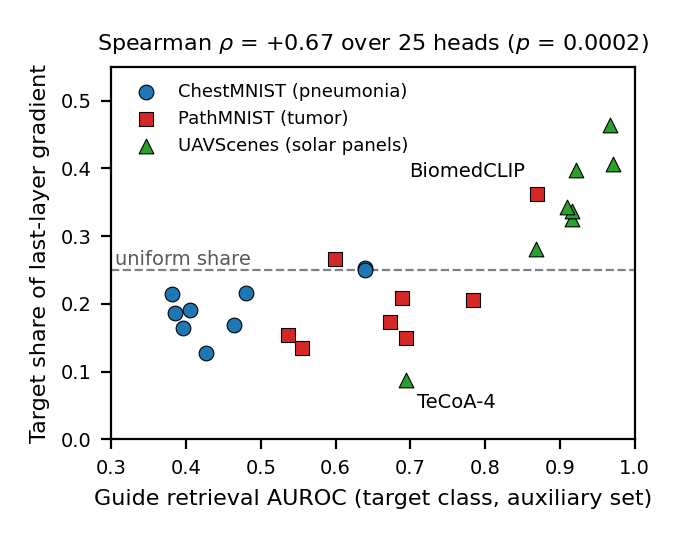
\includegraphics[width=\linewidth]{fig/retrieval_vs_share}
\caption{\textbf{The rigged head selects its targets only when the guide retrieves them.} One point per guide head (ResNet-18 client, 25 heads over three datasets): the AUROC with which the guide's query similarity ranks the target class on the attacker's auxiliary set, against the share of the client's last-layer gradient that the two target images of the private batch receive. Uniform share is 0.25. ChestMNIST guides all sit below 0.65 AUROC and no head selects; the one UAV guide that fails retrieval (TeCoA-4) is the one UAV head that does not select.}
\label{fig:retrieval}
\end{figure}

\begin{table}[t]
\centering
\small
\caption{\textbf{What the rigged head does to the private batch.} For each dataset and guide, the share of the client's last-layer gradient norm that the two target images receive (uniform $=0.25$), the head's mean loss on the targets over its loss on the other six images, and the guide's retrieval AUROC for the target class on the auxiliary set. ResNet-18 client, held-out batch, one head per guide.}
\label{tab:profile}
\begin{tabular}{llccc}
\toprule
Dataset & Guide & AUROC & Target share & Loss ratio \\
\midrule
\multirow{4}{*}{ChestMNIST} & BiomedCLIP & 0.64 & 0.249 & 2.4$\times$ \\
 & CLIP & 0.48 & 0.216 & 0.8$\times$ \\
 & best robust (FARE-2) & 0.38 & 0.214 & 0.9$\times$ \\
 & worst robust (TeCoA-2) & 0.43 & 0.127 & 0.5$\times$ \\
\midrule
\multirow{4}{*}{PathMNIST} & BiomedCLIP & 0.87 & \textbf{0.362} & 1.9$\times$ \\
 & CLIP & 0.60 & 0.266 & 0.4$\times$ \\
 & TeCoA-4 & 0.78 & 0.205 & 0.2$\times$ \\
 & SimCLIP-2 & 0.56 & 0.135 & 0.2$\times$ \\
\midrule
\multirow{4}{*}{UAVScenes} & CLIP & 0.92 & \textbf{0.338} & 2.1$\times$ \\
 & SimCLIP-2 & 0.97 & \textbf{0.464} & 9.5$\times$ \\
 & FARE-2 & 0.97 & \textbf{0.406} & 9.3$\times$ \\
 & TeCoA-4 & 0.69 & 0.087 & 0.02$\times$ \\
\bottomrule
\end{tabular}
\end{table}

\geminio's own diagnostic, the loss ratio on the auxiliary set, says that every head we trained is rigged: 8--14$\times$ on ChestMNIST, 17--28$\times$ on PathMNIST, 19--131$\times$ on UAV.
The private batch tells a different story (\cref{tab:profile}; full table in the supplement).
On UAV, seven of eight guide heads place more than the uniform share of the last-layer gradient on the two solar-panel images (0.28--0.46), with the targets' own-label probability driven down to 0.22--0.39 against 0.48--0.80 for the rest.
The exception is TeCoA-4, the one UAV guide whose query similarity fails to rank solar panels (AUROC 0.69 against 0.87--0.97 for the others): its head puts 0.087 of the gradient on the targets and makes them the \emph{easiest} images in the batch.
On ChestMNIST no head exceeds the uniform share. The BiomedCLIP heads sit exactly at it (0.249, 0.253); every CLIP-family head is below it (0.13--0.22), and the robust-guide heads reach per-image losses of 250--860 on every image of the batch, targets and non-targets alike.
On PathMNIST only the BiomedCLIP head, the one guide with AUROC above 0.75, selects the tumor images (0.362); the seven CLIP-family heads, with AUROC 0.54--0.78, place 0.13--0.27 on them.

Across the 25 heads the target share follows retrieval: Spearman $\rho=0.67$ ($p=.0002$); within UAV, $\rho=0.90$.
Split at 0.75 AUROC, 8 of 9 heads above the threshold select their targets (median share 0.34) and 2 of 16 below it do (median 0.18).
The same holds for the ViT-L client, where the rigged head puts 0.52 of the gradient on the UAV targets (7 of 7 encoders) but 0.15 on the \pneu images, below the uniform share and below its own honest head (0.29).

This resolves the medical result end to end. Vanilla CLIP and all six robust CLIPs rank \pneu at or below chance on the ChestMNIST auxiliary set (any-label AUROC 0.42--0.49, base rate 1.2\%), and the top-ranked auxiliary images under every guide are mostly ``normal'' radiographs no closer in \lpips to the held-out targets than random ones.
A head trained by \cref{eq:geminio} to amplify whatever the guide scores highly therefore learns to amplify a non-\pneu subset, and on the private batch the \pneu images receive no amplification.
Reconstruction then has nothing to select: no ChestMNIST configuration in this study, across two client architectures, 24 queries, eight guides and three reconstruction algorithms, reaches a target \lpips below the 95th percentile of eight random draws from the dataset (best 0.377 against a reference of 0.327 [0.294, 0.361]).
Part of this is the metric, since 64\,px radiographs upscaled to 224\,px are mutually similar under \lpips; the selection failure is not, and it is measured before any reconstruction runs.
\TODO{PathMNIST: does the BiomedCLIP head's 0.36 share turn into selectivity above the reference and target \lpips below it? Group A, Nov 2.}

\subsection{Robust client backbones reveal what the head selects}
\label{sec:backbone}
% results/client_encoder/summary.md, results/client_encoder_plain/summary.md, results/client_encoder_swap_qair_qeff/summary.md,
% results/plain_head/README.md (limits), results/complementarity/private_batch_profile.md

\begin{figure*}[t]
\centering
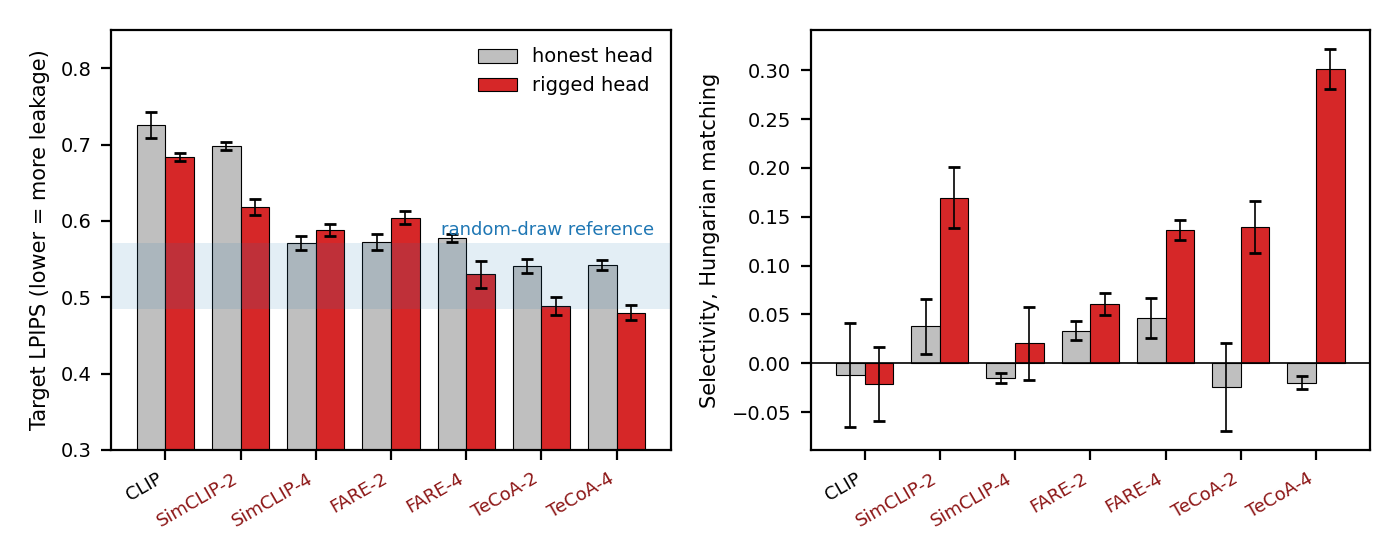
\includegraphics[width=\textwidth]{fig/backbone_uav}
\caption{\textbf{Client backbone and head type on UAV.} Target \lpips (left; shaded band is the 5th--95th percentile of the random-draw reference) and Hungarian selectivity (right) for each ViT-L client encoder under an honest head and under the head rigged for solar panels; mean and standard error over three seeds. Robust encoders in red on the axis. The honest head is never selective; the rigged head is selective only on robust encoders, increasingly with robustness level. \TODO{add the three non-robust comparators when their runs finish.}}
\label{fig:backbone}
\end{figure*}

\begin{table}[t]
\centering
\small
\caption{\textbf{Client backbone, UAV solar-panel targets.} Target \lpips (lower is more leakage) and selectivity (non-target minus target \lpips) under the rigged head and under an honest head on the same frozen encoder, mean over three seeds; $\Delta$ is paired against vanilla CLIP under the rigged head. Hungarian selectivity in parentheses. The bottom block adds encoders that were never adversarially trained. \TODO{comparator rows from results/nov-runs}}
\label{tab:backbone}
\begin{tabular}{lcccc}
\toprule
 & \multicolumn{2}{c}{Rigged head} & \multicolumn{2}{c}{Honest head} \\
\cmidrule(lr){2-3}\cmidrule(lr){4-5}
Encoder & Target \lpips & Selectivity & Target \lpips & Selectivity \\
\midrule
CLIP (OpenAI) & 0.683 & $-$0.007 ($-$0.02) & 0.726 & $-$0.000 \\
SimCLIP-2 & 0.618 & +0.036 (+0.17) & 0.698 & +0.02 \\
SimCLIP-4 & 0.589 & +0.025 (+0.02) & 0.571 & $-$0.01 \\
FARE-2 & 0.604 & +0.032 (+0.06) & 0.572 & +0.01 \\
FARE-4 & 0.530 & +0.067 (+0.14) & 0.578 & $-$0.01 \\
TeCoA-2 & 0.489 & +0.092 (+0.14) & 0.541 & $-$0.00 \\
TeCoA-4 & \textbf{0.480} & \textbf{+0.122} (+0.30) & 0.542 & +0.01 \\
\midrule
CLIP (LAION-2B) & \TODO{} & & & \\
DINOv2 & \TODO{} & & & \\
ViT-L/16 IN-21k & \TODO{} & & & \\
\midrule
ResNet-18 & 0.476 & +0.114 (+0.20) & -- & -- \\
\bottomrule
\end{tabular}
\end{table}

On UAV, where the head selects, all six adversarially fine-tuned ViT-L backbones leak the targets more than vanilla CLIP (paired $p\le.019$, 6 of 6), the effect is ordered by robustness level within each family ($\epsilon=4$ leaks more than $\epsilon=2$), and the gain on the query-matched images is 1.5--3 times the gain on the rest, so selectivity rises from zero to +0.12 (+0.30 under one-to-one matching) on TeCoA-4 (\cref{tab:backbone}).
Only TeCoA-4's target \lpips (0.480) falls below the 5th percentile of the random-draw reference (0.485); the rest of the robust encoders sit inside or above it.

Three controls separate the two factors.
\emph{Honest head}: trained with the mean loss on the same frozen encoders, it gives selectivity within $\pm0.02$ on all seven encoders, and the paired drop from the rigged head is significant on 5 of 7 (Wilcoxon over encoders $p=.031$).
Yet the honest head still reconstructs robust encoders' batches better than CLIP's (target \lpips 0.54--0.70 against 0.73; 5 of 6 encoders, $p\le.02$): invertibility is a property of the backbone that exists without rigging, and the rigged head adds only +0.03 target \lpips on top of it.
\emph{Swapped query}: rigging the head for airport runways instead of solar panels on the same batch removes the solar selectivity (6 of 7 encoders, $p=.031$) and raises solar target \lpips on 7 of 7 while leaving non-targets unchanged; the selectivity is a property of the query, not of rigging in general.
\emph{Gradient share}: the rigged head puts 0.52 of the last-layer gradient on the two targets (0.37--0.69 across the seven encoders), the honest head 0.15 and the runway head 0.10, with the runway images then taking 0.28--0.66.
Low confidence on the matched images and a concentrated gradient appear together, and only under the head rigged for them.

Two things these controls do not show.
The ``interaction'' between head and backbone, positive on all six robust encoders, is measured against a single non-robust comparator, so the bottom block of \cref{tab:backbone} adds three ViT-L encoders that were trained without adversarial fine-tuning. \TODO{state what they show: if LAION-2B CLIP, DINOv2 and the supervised ViT-L invert as well as the robust CLIPs, the effect is about the encoder family rather than robustness; if not, it is specific to adversarial fine-tuning.}
And on ChestMNIST every ViT-L client fails regardless of robustness (target \lpips 0.76--0.87; honest head 0.67--0.87), which \cref{sec:selection} attributes to the head never selecting the targets rather than to the backbone.

\subsection{Robust guides change reconstruction quality, not selection}
\label{sec:guide}
% results/heldout_rerun/summary.md block 2 (medical_vlm*_ho, uav_vlm*_ho), results/complementarity/vlm_retrieval.md,
% aux_appearance.md; PathMNIST guide table pending (results/nov-runs/pathmnist-resnet)

\begin{table}[t]
\centering
\small
\caption{\textbf{Guide VLM, ResNet-18 client.} Target \lpips, mean over three seeds, with the paired difference against vanilla CLIP as the guide; negative means a stronger attack. BiomedCLIP is the domain guide for the medical datasets. \TODO{PathMNIST column from results/nov-runs/pathmnist-resnet}}
\label{tab:guide}
\begin{tabular}{lcccccc}
\toprule
 & \multicolumn{2}{c}{ChestMNIST} & \multicolumn{2}{c}{PathMNIST} & \multicolumn{2}{c}{UAVScenes} \\
\cmidrule(lr){2-3}\cmidrule(lr){4-5}\cmidrule(lr){6-7}
Guide & \lpips & $\Delta$ & \lpips & $\Delta$ & \lpips & $\Delta$ \\
\midrule
BiomedCLIP & 0.590 & $-$0.10 & \TODO{} & & -- & -- \\
CLIP & 0.687 & -- & & -- & 0.470 & -- \\
SimCLIP-2 & 0.448 & $-$0.24 & & & 0.473 & +0.00 \\
SimCLIP-4 & 0.444 & $-$0.24 & & & 0.565 & +0.10 \\
FARE-2 & \textbf{0.377} & $-$0.31 & & & 0.515 & +0.04 \\
FARE-4 & 0.491 & $-$0.20 & & & 0.562 & +0.09 \\
TeCoA-2 & 0.411 & $-$0.28 & & & 0.496 & +0.03 \\
TeCoA-4 & 0.419 & $-$0.27 & & & 0.591 & +0.12 \\
\bottomrule
\end{tabular}
\end{table}

When a robust CLIP replaces vanilla CLIP as the guide while the client stays a ResNet-18, the ChestMNIST attack reconstructs the batch better on every robust guide (6 of 6, 18 of 18 seed pairs, sign test $p=8\times10^{-6}$; \cref{tab:guide}), and the ImageNet-robust guides beat the domain guide BiomedCLIP as well.
This is not a targeting effect. \Cref{tab:profile} shows that none of these heads places the uniform share of the gradient on the \pneu images, and non-target \lpips improves by as much as target \lpips (selectivity stays within $\pm0.07$ of zero for all guides).
What changes is the loss regime: the robust-guide heads assign per-image losses two orders of magnitude larger than the vanilla-CLIP head to every image in the batch, which makes the whole gradient easier to invert.
On UAV, where retrieval differs by guide, there is no robust-guide effect on average (6 of 18 seed pairs), but retrieval precision tracks attack strength across the seven guides ($\rho=-0.86$, $p=.014$), and the guide that fails retrieval (TeCoA-4) gives the weakest attack.
\TODO{PathMNIST: guide retrieval spreads 0.54--0.87 here, so this is the cleanest test of retrieval against attack strength within one dataset.}

\subsection{Where the attack fails}
\label{sec:failure}
% results/heldout_rerun/summary.md block 3 (24-query sweep) and block 4 (floor conditions); abstract.tex comment (3)

Across 12 query variants per domain (table in the supplement), the ChestMNIST attack is strongest with a misspelled query (target \lpips 0.40) and a purely negated one (0.46), close to the base query (0.51) with a Spanish translation (0.53), and breaks with an exclusion (``not pneumonia'', 0.67), a disjunction (0.70), a terse one-word query (0.71) and an indirect description (0.93).
On UAV every variant lands between 0.44 and 0.54.
Misspelling, translation and negation therefore do not weaken the attack, because the guide's embedding absorbs them; what weakens it is a query whose embedding no longer retrieves the class.
Four further conditions are floors rather than findings: ChestMNIST at batch 32, BatchNorm in training mode, GradInversion on ChestMNIST and the indirect query all leave the undefended attack at target \lpips $\ge0.7$, consistent with Valadi \etal~\cite{valadi2025feasibility}, so no defense result should be read from them.
